\section{Experiments}
brief overview of the experiments/models

\subsection{Random forest}
% https://www.tensorflow.org/decision_forests
TensorFlow Decision Forests (TF-DF) is the library used to train and evaluate the random forest model.

% (https://www.stat.berkeley.edu/~breiman/randomforest2001.pdf)
A Random Forest is a collection of deep CART decision trees trained independently and without pruning.
Each tree is trained on a random subset of the original training dataset (sampled with replacement).
The algorithm is unique in that it is robust to overfitting, even in extreme cases e.g. when there are more features than training examples.
It is probably the most well-known of the Decision Forest training algorithms.

\subsubsection{Features}
We need to adjust the dataset because the Random Forest model does not accept time series or multivariate data as input.

\begin{figure}[!htbp]
  \begin{subfigure}{.5\textwidth}
    \centering
    \[
      \begin{blockarray}{ccccc}
        & b_0 & b_1 & \dots & b_{15} \\
        \begin{block}{c|cccc|}
          t_0 & 0.2 & 1.6 & \dots & 1.7  \\
          t_1 & 1.3 & 1.8 & \dots & 1.8 \\
          \vdots & \vdots & \vdots &  & \vdots   \\
          t_{53} & 0.6 & 0.4 & \dots & 1.3 \\
        \end{block}
      \end{blockarray}
    \]
    \caption{One observation in a 2-dim array}
    \label{fig:figtrans1}
  \end{subfigure}%
  \begin{subfigure}{.5\textwidth}
    \centering
    \[
      \begin{blockarray}{cc}
      \begin{block}{c|c|}
        t_0::b_0 & 0.2 \\
        t_0::b_1 & 1.6 \\
        \vdots & \vdots \\
        t_{53}::b_{15} & 1.3 \\
      \end{block}
      \end{blockarray}
    \]
    \caption{Forged features for Random forest}
    \label{fig:figtrans2}
  \end{subfigure}
  \caption{Transformation of one observation from a 2-dim array to a 1-dim array}
  \label{fig:figtrans}
\end{figure}

As shown in Figure \ref{fig:figtrans1}, each sample is initially represented by a 2-dimensional array of size (54, 16), where 16 bands capture the pixel's characteristics and 54 time steps reflect its progression. 
However, through the transformation process, the representation is transformed into a more 1-dimensional array of size (864, 1) as depicted in Figure \ref{fig:figtrans2}. 

The model's training utilizes the new representation of the data, composed of 864 derived features, to generate 300 trees.
The performance of each tree is then summarized in Table \ref{tab:rfresults}, which displays the number of nodes, the number of features utilized, and the overall accuracy

\begin{table}[!htbp]
  \centering
    \begin{tabular}{lrrr}
    Model                       & Nodes   & Used features & Overall Accuracy             \\[0.2cm] 
    \hline \\[-0.2cm]
    Imputed missing values      & 523,636  & 753          & $91.03 \pm 0.42$\\
    Not imputed missing values  & 519,932  & 718          & $89.72 \pm 0.84$
    \end{tabular}
  \caption{Random forest results}
  \label{tab:rfresults}
\end{table}


\subsection{TempCNN}
%- paper overview
"Temporal Convolutional Neural Network for the Classification of Satellite Image Time Series" article \cite{tempCNN} presents a machine learning model for classifying satellite image time series data.
The model is based on Convolutional Neural Networks (CNNs) and aims to improve upon traditional image classification methods by incorporating time-series information into the model.

The model inputs a series of satellite images, which are transformed into a compact representation, and uses a series of convolutional and pooling operations to extract high-level features from the data.
The article introduces a novel approach to classifying satellite image time series data and highlights the potential applications of the model in fields such as remote sensing and environmental monitoring.

- temporal convolutional layer

- data preparation

-- guidance


\subsubsection{Model}

\begin{figure}[!htbp]
  \centering
  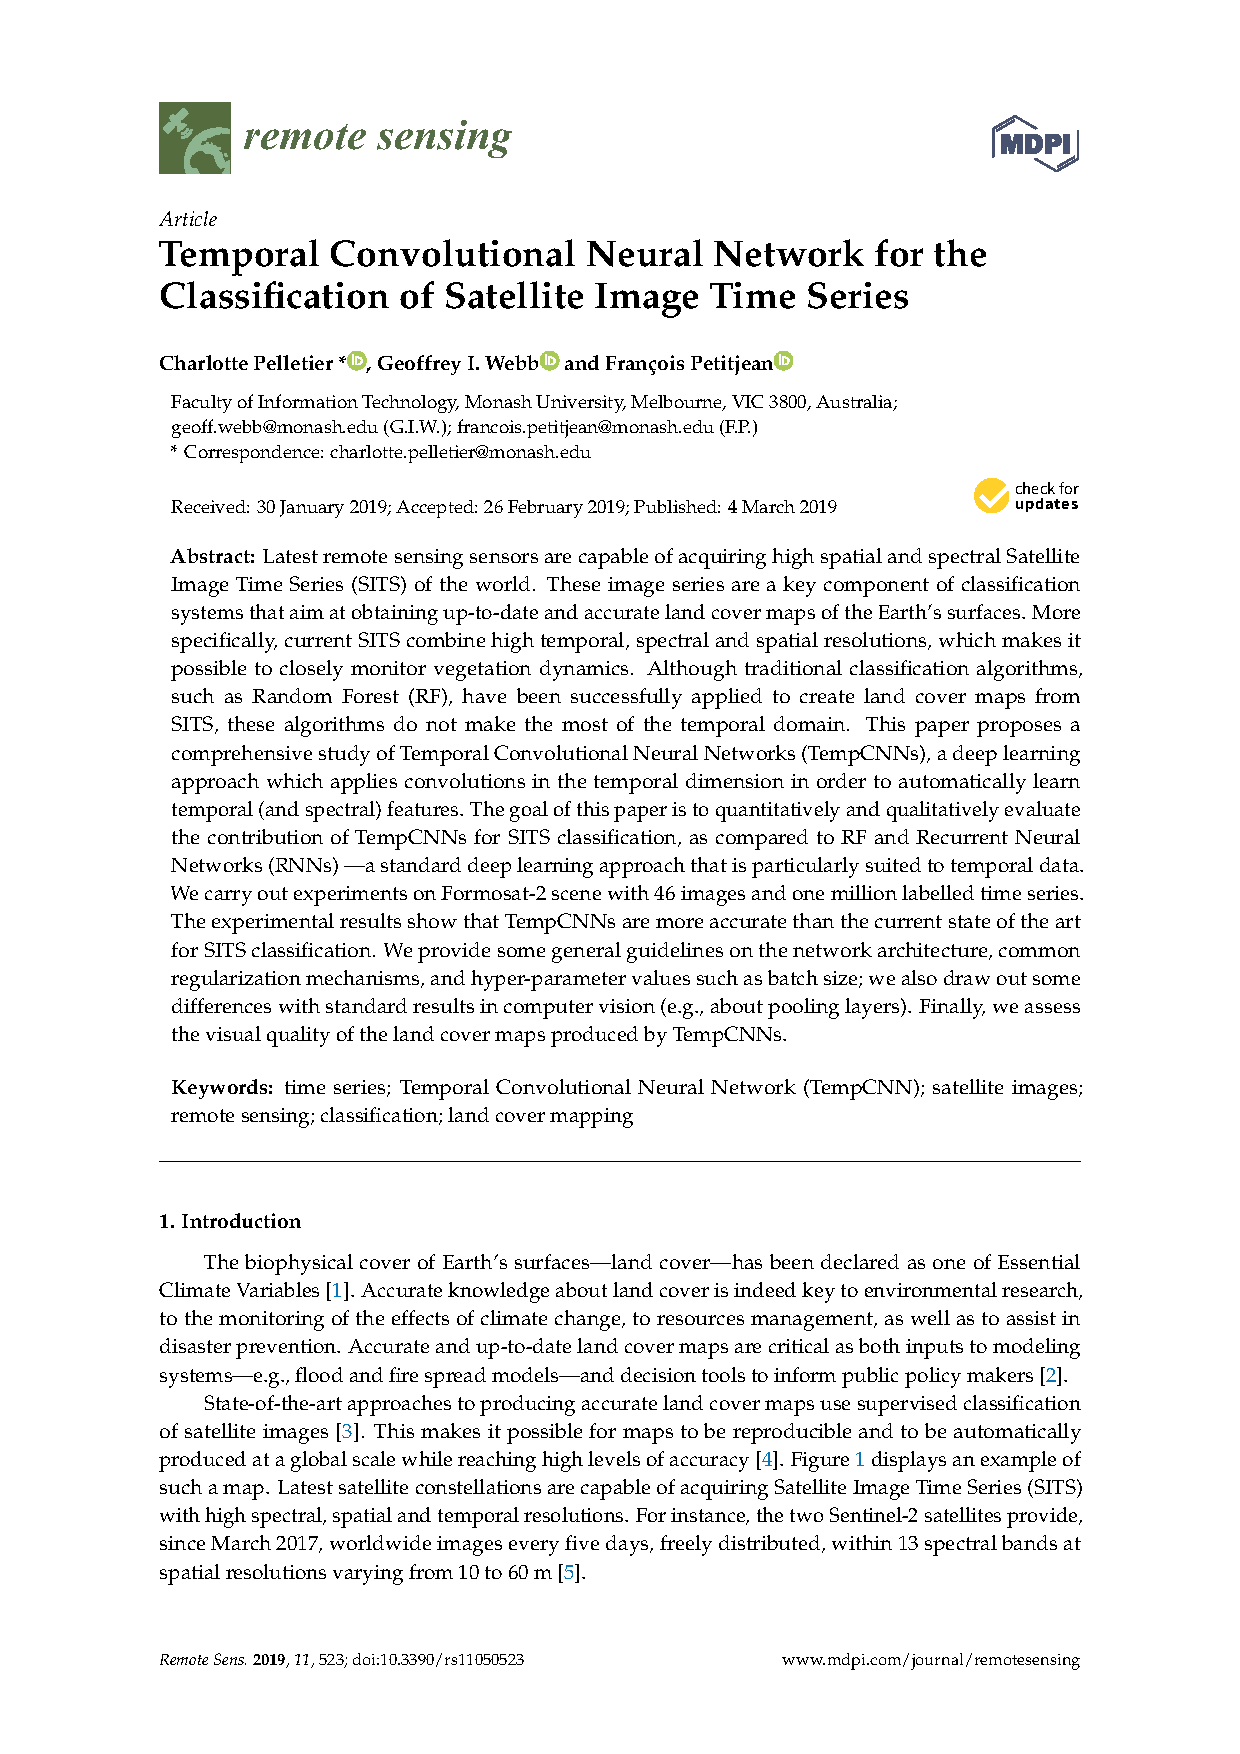
\includegraphics[width=1\textwidth]{tempCNN}
  \caption{The TempCNN model \cite{tempCNN}}
\end{figure}

- description

- regularization

- filter size

\subsubsection{Experimental results}




- influence of depth

\begin{table}[!htbp]
  \centering
   \begin{tabular}{rclrr}
   Model&&                  & No imputation         & Pre imputation             \\[0.2cm]
   \hline \\[-0.2cm]
    1CONV256 &+& 1FC64   	 & $93.01 \pm 0.97$ 	 & $92.80 \pm 0.65$\\
    2CONV128 &+& 1FC128  	 & $93.50 \pm 1.81$ 	 & $\mathbf{92.97 \pm 2.05}$\\
    3CONV64 &+& 1FC256   	 & $\mathbf{93.45 \pm 1.36}$ 	 & $91.29 \pm 1.18$\\
    4CONV32 &+& 1FC512   	 & $91.89 \pm 2.10$ 	 & $88.94 \pm 1.34$\\
    5CONV16 &+& 1FC1024  	 & $90.66 \pm 1.21$ 	 & $86.54 \pm 2.00$\\
    6CONV8 &+& 1FC2048   	 & $86.74 \pm 3.71$ 	 & $87.95 \pm 2.22$\\
    &&1FC5115          	 & $89.64 \pm 0.48$ 	 & $90.78 \pm 1.69$\\
   \end{tabular}
   \caption{depth}
 \end{table}

 - influence of width

 \begin{table}[!htbp]
  \centering
   \begin{tabular}{rclrr}
   Model&&                  & No imputation         & Pre imputation             \\[0.2cm]
   \hline \\[-0.2cm]
    3CONV16 &+& 1FC256    	 & $92.64 \pm 0.01$ 	 & $91.69 \pm 0.12$\\
    3CONV32 &+& 1FC256    	 & $\mathbf{93.88 \pm 0.76}$ 	 & $91.78 \pm 0.53$\\
    3CONV64 &+& 1FC256    	 & $92.48 \pm 2.01$ 	 & $92.72 \pm 0.38$\\
    3CONV256 &+& 1FC256   	 & $91.32 \pm 3.22$ 	 & $91.47 \pm 0.51$\\
    3CONV512 &+& 1FC256   	 & $90.96 \pm 5.13$ 	 & $92.40 \pm 0.70$\\
    3CONV1024 &+& 1FC256  	 & $92.87 \pm 2.33$ 	 & $\mathbf{93.40 \pm 0.37}$\\
   \end{tabular}
   \caption{complexity}
 \end{table}

- batch-size

\begin{table}[!htbp]
  \centering
   \begin{tabular}{lrr}
   batchsize                  & No imputation         & Pre imputation             \\[0.2cm]
   \hline \\[-0.2cm]
    16  	 & $91.92 \pm 1.50$ 	 & $92.16 \pm 2.75$\\
    32  	 & $\mathbf{91.61 \pm 1.99}$ 	 & $\mathbf{93.74 \pm 0.03}$\\
    64  	 & $90.88 \pm 2.63$ 	 & $92.30 \pm 2.89$\\
    128  	 & $91.54 \pm 2.99$ 	 & $91.52 \pm 1.67$\\
   \end{tabular}
   \caption{batchsize 3CONV64+1FC256}
 \end{table}

- imputation vs no imputation

\pagebreak
\subsection{AJ-RNN}
- model overview

- GRU vs LSTM (running)

- learnig rate
- batch size 

\subsubsection{Light AJ-RNN}
- model overview\\
- baseline

\subsection{L-TAE}
- model overview\\
- PixelSetEncoder\\
- DenseEncoder

- imputation vs no imputation
- tanh

\subsection{Results}

\begin{table}[!htbp]
  \centering
    \begin{tabular}{lrrr}
    Model                       & Overall Accuracy             \\[0.2cm] 
    \hline \\[-0.2cm]
    RF      & $91.03 \pm 0.42$
    \end{tabular}
  \caption{Overall accuracy of the models with pre imputed missing values} 
\end{table}

\begin{table}[!htbp]
  \centering
    \begin{tabular}{lrrr}
    Model                       & Overall Accuracy             \\[0.2cm] 
    \hline \\[-0.2cm]
    RF  & $89.72 \pm 0.84$
    \end{tabular}
  \caption{Overall accuracy of the models with missing values} 
\end{table}